\documentclass[a4paper,12pt]{article}
\usepackage[english]{babel}
\usepackage[utf8]{inputenc}
\usepackage{amssymb}
\usepackage{amsmath}
\usepackage{mathtools}
\usepackage{listings, lstautogobble}
\usepackage{tikz}
\usepackage{graphicx}
\graphicspath{ {./images/} }
\usepackage{xcolor}
\usepackage{array}
\usepackage{hyperref}
\hypersetup{
    colorlinks=true,
    linkcolor=blue,
    filecolor=magenta,      
    urlcolor=cyan,
}

\urlstyle{same}

\definecolor{RoyalBlue}{cmyk}{1, 0.50, 0, 0}

% Code listing init
\lstset{
  keywordstyle=\color{RoyalBlue},
  basicstyle=\scriptsize\ttfamily,
  commentstyle=\ttfamily\itshape\color{gray},
  stringstyle=\ttfamily,
  showstringspaces=false,
  breaklines=true,
  frameround=ffff,
  frame=single,
  language=bash,
  rulecolor=\color{black},
  autogobble=true
}

\pagestyle{headings}

\begin{document}

\markright{Entropass}
%%%%%%%%%%%%%%%%%%%%%%%%%%%%%%%%%%%%%%%%%%%%%%%%%%%%%%%%%%%%%%%%%%%%%%%%%%%%%%%%
%%%%%%%%%%%%%%%%%%%%%%%%%%%%%%%%%%%%%%%%%%%%%%%%%%%%%%%%%%%%%%%%%%%%%%%%%%%%%%%%
%%%%%%%%%%%%%%%%%%%%%%%%%%%%%%%%%%%%%%%%%%%%%%%%%%%%%%%%%%%%%%%%%%%%%%%%%%%%%%%%
\begin{titlepage}
  % \maketitle
  \begin{center}
    \vspace*{1cm}

    \Huge
    \textbf{EntroPass}

    \vspace{0.5cm}
    \LARGE
    \textbf{Research Report}


    \Large
    A research report presented for the design \& implementation of EntroPass\\
    \normalsize
    Flexible Project

    \vspace{0.8cm}

    
\includegraphics[width=0.9\textwidth]{entropass}

  \end{center}
  \vfill  
  \vspace{1.5cm}

  \textbf{Jochem Stevense}\\
  \normalsize
  Embedded Systems Engineering\\
  Flexible Project\\
  HAN University of Applied Science\\
  Ton Ammerlaan, Remko Welling\\
  The Netherlands\\
  2021\\
  Version 0.1
\end{titlepage}

\thispagestyle{plain}
\begin{center}
    \Large
    \textbf{Research Report}
        
    \vspace{0.4cm}
    \large
    Entropass
        
    \vspace{0.4cm}
    \textbf{Jochem Stevense}
       
    \vspace{0.9cm}
    \textbf{Abstract}
\end{center}

This research report is created for the HAN University of Applied Science as part of the Bachelor Flexible Project of Jochem Stevense and investigates the possibilities of developing a tool to efficiently generate password word-lists, where a specific person is targeted. The purpose of this tool is to show users the vulnerabilities of using memorable passwords in a very practical manner. Additionally, the tool is to be used purely for legal purposes, such as penetration testing.\\

Word-lists are often used to perform dictionary attacks against services that require authentication. These word-lists are mostly a compilation of most used passwords, resulting from numerous data-leaks, and do not target a specific person. This is useful when trying to perform these attacks on a larger number of targets. However, when targeting a single target, these passwords can be too general, which is why this research aims to lay the foundations for a tool that generates word-lists based on provided personal information of a single target. To do this, research had to be conducted to password practices, which resulted in the following research question:\\
\textit{What functionalities should a password word-list generating tool have to be able to utilise standard password practices when targeting a single, specific user?}\\
This research resulted in indications about the most used password formats, characters, and personal information used to create memorable passwords.\\
The research also provided insights to how the data might be processed and structured for efficient dictionary attacks, resulting in two methods; generating the maximum amount of passwords with given personal information and scoring them according to the most popular formats, characters and personal information, and generating far less passwords, only sticking to the most popular formats and scoring these passwords based on the same criteria as the first method. Both of these methods have their advantages and disadvantages, where the first method is most likely to produce the right password, it is also computationally demanding. The second method on the other hand is far less demanding, but less likely to produce the right results.\\
To keep the program up to date, the research had to be capable of being done automatically, so the program can do this on demand, resulting in an automated update script.\\

The password formats, characters and used personal information is used to score passwords and the data will be allowed to be processed and structured according to either one of the mentioned methods, based on the configuration, to allow for the program to be adjusted, based on the use-case.\\
The program will be updated on password formats and characters by using the automated update script, but it is recommended to also research and develop a way to automate the categorising of the personal information used in passwords, although this could prove challenging and would require a large amount of data.

\newpage
  
%%%%%%%%%%%%%%%%%%%%%%%%%%%%%%%%%%%%%%%%%%%%%%%%%%%%%%%%%%%%%%%%%%%%%%%%%%%%%%%%
\tableofcontents

\newpage
%%%%%%%%%%%%%%%%%%%%%%%%%%%%%%%%%%%%%%%%%%%%%%%%%%%%%%%%%%%%%%%%%%%%%%%%%%%%%%%%
\section{Introduction}
\label{ch:intro}
This research report has been created for the HAN University of Applied Science as part of the Bachelor Flexible Project of Jochem Stevense and investigates the possibilities of developing a tool to efficiently guess for passwords and write them into a word-list, targeting a single specific person. The purpose of such a tool is to show users the vulnerabilities introduced by using memorable passwords and to generate word-lists to be used for ethical hacking and penetration testing purposes.\\

Word-lists are used by threat actors to perform dictionary attacks on services that require authentication, parsing through a list of words and trying to login, using these words as passwords. The same can be done with usernames, although usernames are generally easier to discover, depending on the service to authenticate to. Most of the available word-lists are simply a compilation of previously discovered passwords, resulting from data breaches, and often hold the most used ones or the ones found in a specific data breach. This can prove useful when targeting a large number of users, since it is likely that one of these users will use a password that is included in the list. However, when targeting a single user, the odds of the password being included in such a list can be small. The reason for this is that many users use personalised passwords to be able to memorise the credentials. Although these personalised passwords are unlikely to be included in a general word-list, they are often not hard to guess, when personal information about a target user is known.\\
This research aims to gain insight into what functionality a password word-list generating tool would need, to be able to guess these personalised passwords for a single user. To reach this goal, the following research question has been defined:\\

\textit{What functionalities should a password word-list generating tool have to be able to utilise standard password practices when targeting a single, specific user?}

The main research question has been divided into several sub-questions. These sub-questions are the following:

\begin{itemize}
\item \textit{What are standard password formats?}
\item \textit{What personal information is relevant for password guessing?}
\item \textit{How can the processed information be structured efficiently, to allow for efficient dictionary attacks?}
\item \textit{How can the program remain up to date with changing password practices?}
\end{itemize}

This research consisted of a combination of qualitative and quantitative research to find the most used password formats, used personal information for passwords, how the information could be structured and how to remain up to date with changing password practices. Desk research has been used to find the most used password formats, by gathering publicly available leaked passwords, collected by Daniel Miessler \cite{bib:seclists}, and analysing the passwords for the formats, and most used characters. The found passwords have also been analysed to detect personal information embedded into the passwords. Once this information was found, field research has been used to test the structuring of the data and how to analyse the data automatically and keep up with changing password practices.

\newpage
\section{Research}

\subsection{Password Entropy and Patterns}
Ma, Campbell Tran and Kleeman \cite{bib:entro} mention that password entropy, used to indicate password strength, is loosely defined and mention that the calculation of this entropy is an inadequate indicator to password strength. Password strength is not only defined by the used character library and length, but is also relative to the attacker. Entropy calculations might indicate a password to be very strong, even though the actual entropy is effectively very low if an attacker has accurate ideas on what this password might be.\\

Chou, Lee, Yu, Lai, Huang and Hsueh \cite{bib:pform} define password formats to have certain lengths, a combination of characters, and a pattern in the order of the characters and have proven so with the help of machine learning tools to learn these patterns and reproduce passwords using these patterns. This information allows for a clear direction for the analysing of password formats.

\subsection{Methodology for Password Patterns Research}
The methodology deals with the methods, used to answer the sub-questions and the main question, formulated in chapter \ref{ch:intro}. Firstly, the sub-questions will be handled, after which the main research question will be dealt with.

\begin{itemize}
\item \textit{What are standard password formats?}\\
  To answer this question, desk research was conducted, using online resources, such as leaked data/passwords, to create a list of formats, as used by users in the breach. The formats have been sorted in a list of most used to least used. The passwords have also been analysed for most used characters. This will be done automatically by using a Python script, which was written specifically for the use of this research. The script will be made available for interested parties with the final project.
  
\item \textit{What personal information is relevant for password guessing?}\\
  Passwords are often based on personal information to make them easier to memorise. This personal information was mapped to categories, to determine what a person is most likely to use for a memorable password. This has been done by desk research. This desk research involved the use of the earlier mentioned word-lists from data breaches and analysing these manually to determine what categories are popular amongst users. Categories involve aspects like, relationships, date of birth, pet names, etc.
  
\item \textit{How can the processed information be structured efficiently, to allow for efficient dictionary attacks?}\\
  To be able to answer this question, field research was conducted to test different structures and determine which is most efficient in terms of finding the password as fast as possible.

\item \textit{How can the program remain up to date with changing password practices?}\\
  This question was answered by looking into sources of information for password practices, after which possibilities were researched for gathering this information and analysing it in an automated way.
\end{itemize}

\section{Results}

The results of the research will be handled per question, firstly dealing with the sub-questions. The results are listed in this paragraph. The conclusions from these results will be dealt with in the Conclusions chapter.

\subsection{What are standard password formats?}

To be able to determine patterns in passwords, password formats have been researched. The formats have been defined as the combination of password length, used characters (differentiating between lower case alphabetical, higher case alphabetical, digits and special characters) and the positions of the used characters. To determine the most used password formats, several password files from Daniel Miessler's Seclists \cite{bib:seclists} have been used for analysis, with the help of custom Python scripts. These password files have been the results of disclosed data-breaches and are/were real passwords. The total number of used passwords is 37,045 (thirty seven thousand forty five), and the used files are listed in the Appendices \ref{app:pwordfile}. The total number of characters in the combined files is 294,028.\\

Figure \ref{fig:pform} shows the results of the password analysis, with the X-axis being populated with the discovered password formats, and the Y-axis indicating the number of times these formats have been found. The password formats contain a combination of $d$, $c$, $C$ and $s$. These character have the following meaning:
\begin{itemize}
\item $d=$Digit ($1,2,3,4,...$)
\item $c=$Lower-case Alphabetical character ($a,b,c,d,e,...$)
\item $C=$Higher-case Alphabetical character ($A,B,C,D,E,...$)
\item $s=$Special character ($',/,?,!,...$)
\end{itemize}

\begin{figure}[!ht]
  \centering
  \hspace*{-5.4cm}
  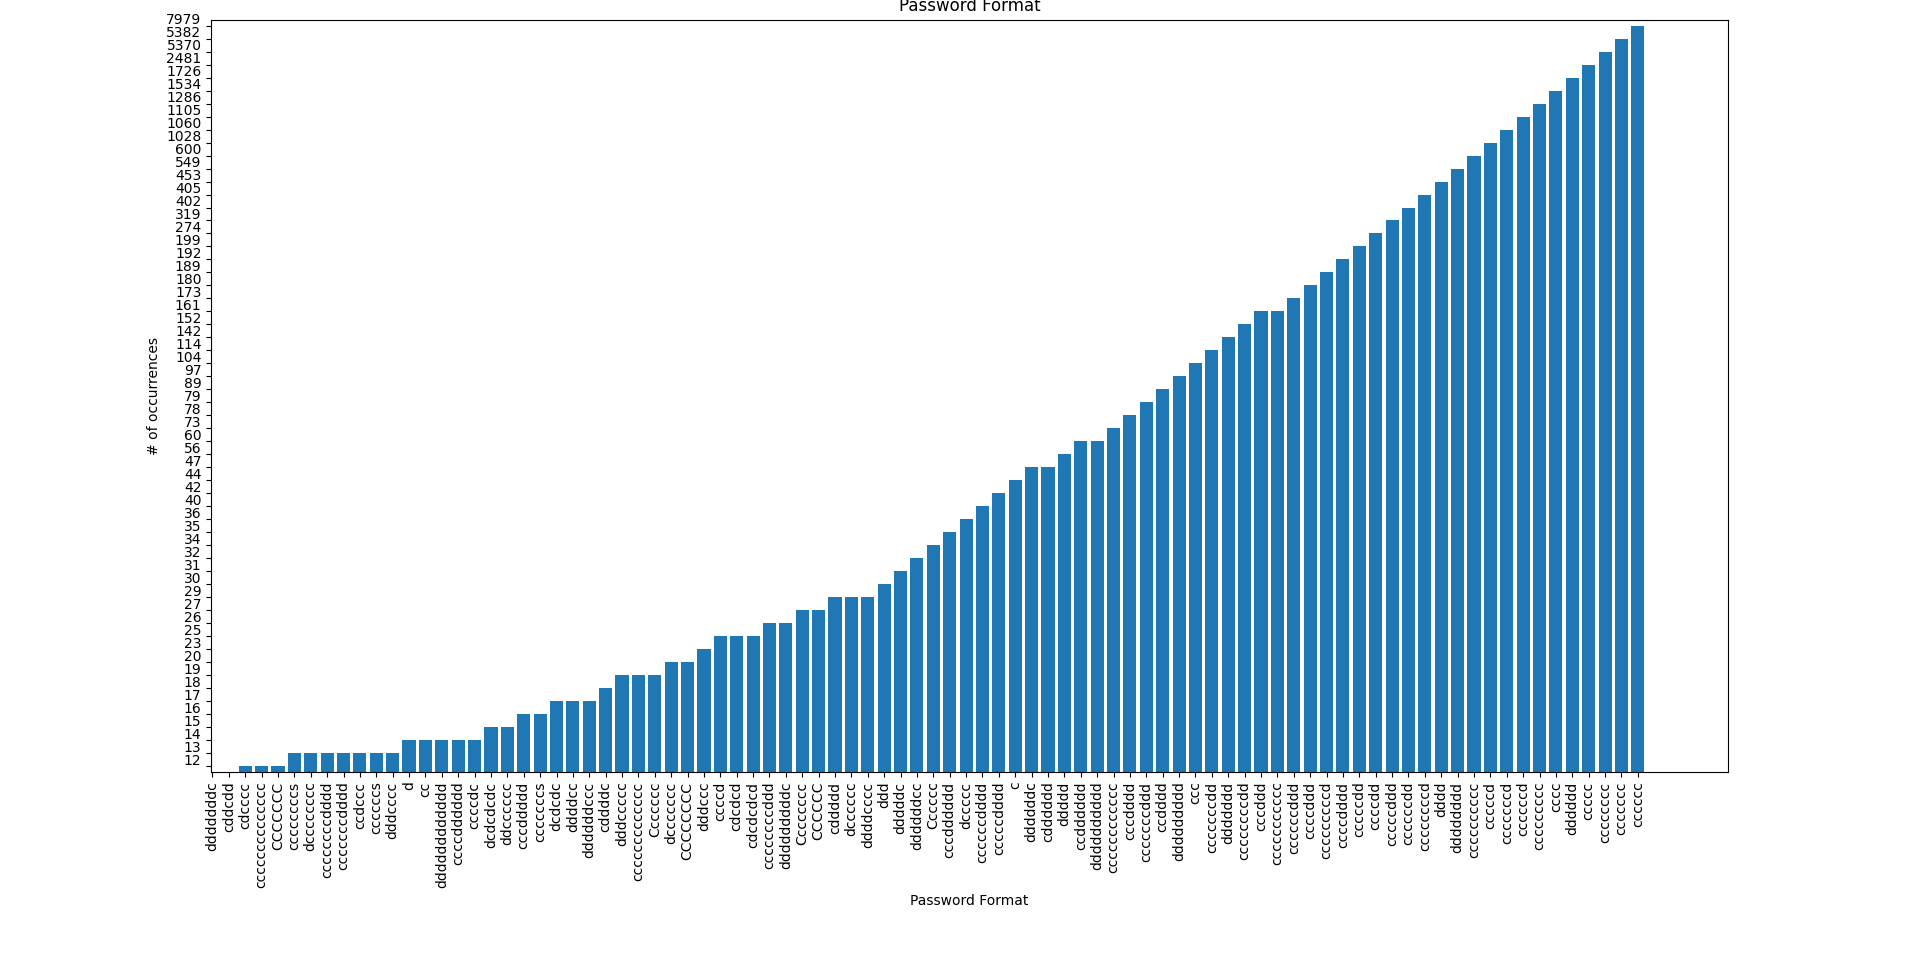
\includegraphics[width=1.8\textwidth]{password_formats}
  \caption{Password Format}
  \label{fig:pform}
\end{figure}

Notable from figure \ref{fig:pform} is that the top four (right most) password formats all consist of lower-case characters and the top seven consist of only one type of character, being lower-case alphabetical characters or digits. Looking further towards the left of the X-axis, this trend mostly holds, with only few combinations with at most two of the four types of characters. More than two types has not been discovered in the data sets. Overall, the lower-case alphabetical characters seem most popular, followed by digits.\\

Further analysis of the passwords can be seen in figure \ref{fig:pchar}. This graph confirms the statement that lower-case alphabetical characters are most popular, followed by digits. Only about halfway on the X-axis do more upper-case alphabetical characters and special characters appear, having at most about 1,200 occurrences in about 294,028 characters.

\begin{figure}[!ht]
  \centering
  \hspace*{-5.4cm}
  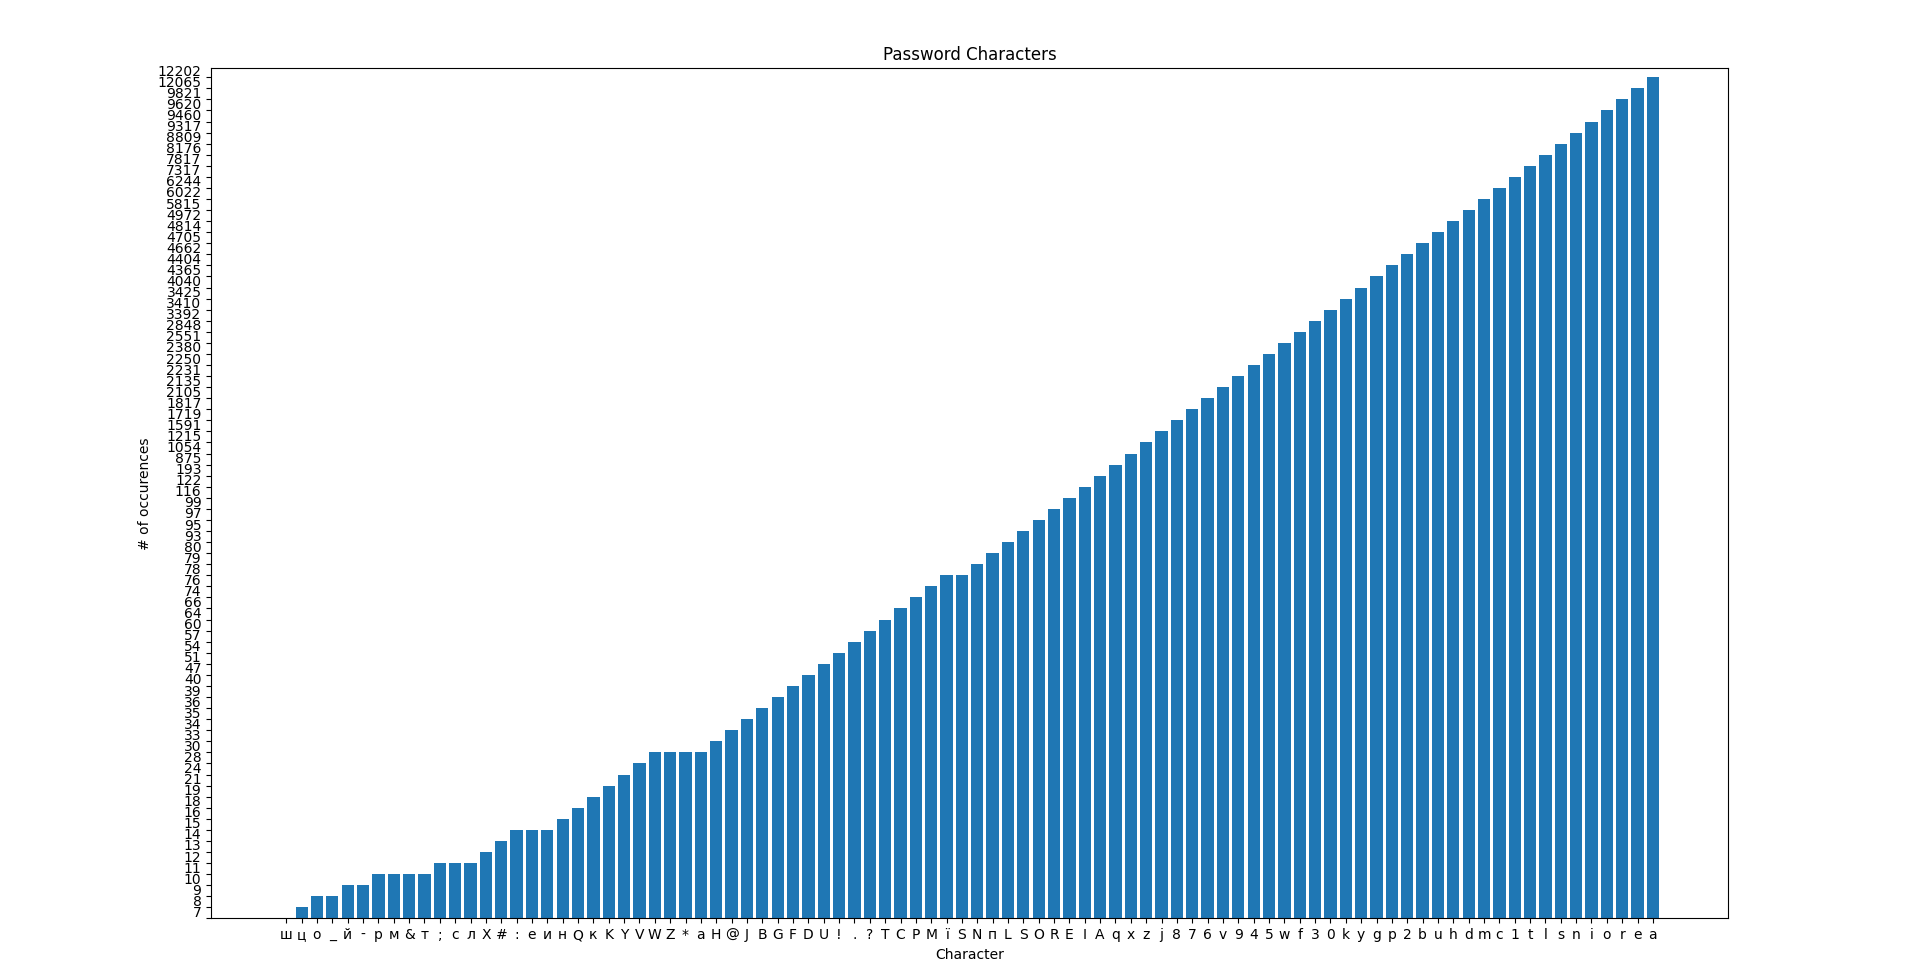
\includegraphics[width=1.8\textwidth]{password_chars}
  \caption{Character Usage}
  \label{fig:pchar}
\end{figure}

Focusing more on the length of the passwords, figure \ref{fig:plen} shows the most used password lengths. Perhaps unsurprisingly, the most used length of six is far from being the longest in the graph. Furthermore, the six most occurring lengths are all under 10, with 10 being the seventh most occurring.

\begin{figure}[!ht]
  \centering
  \hspace*{-5.4cm}
  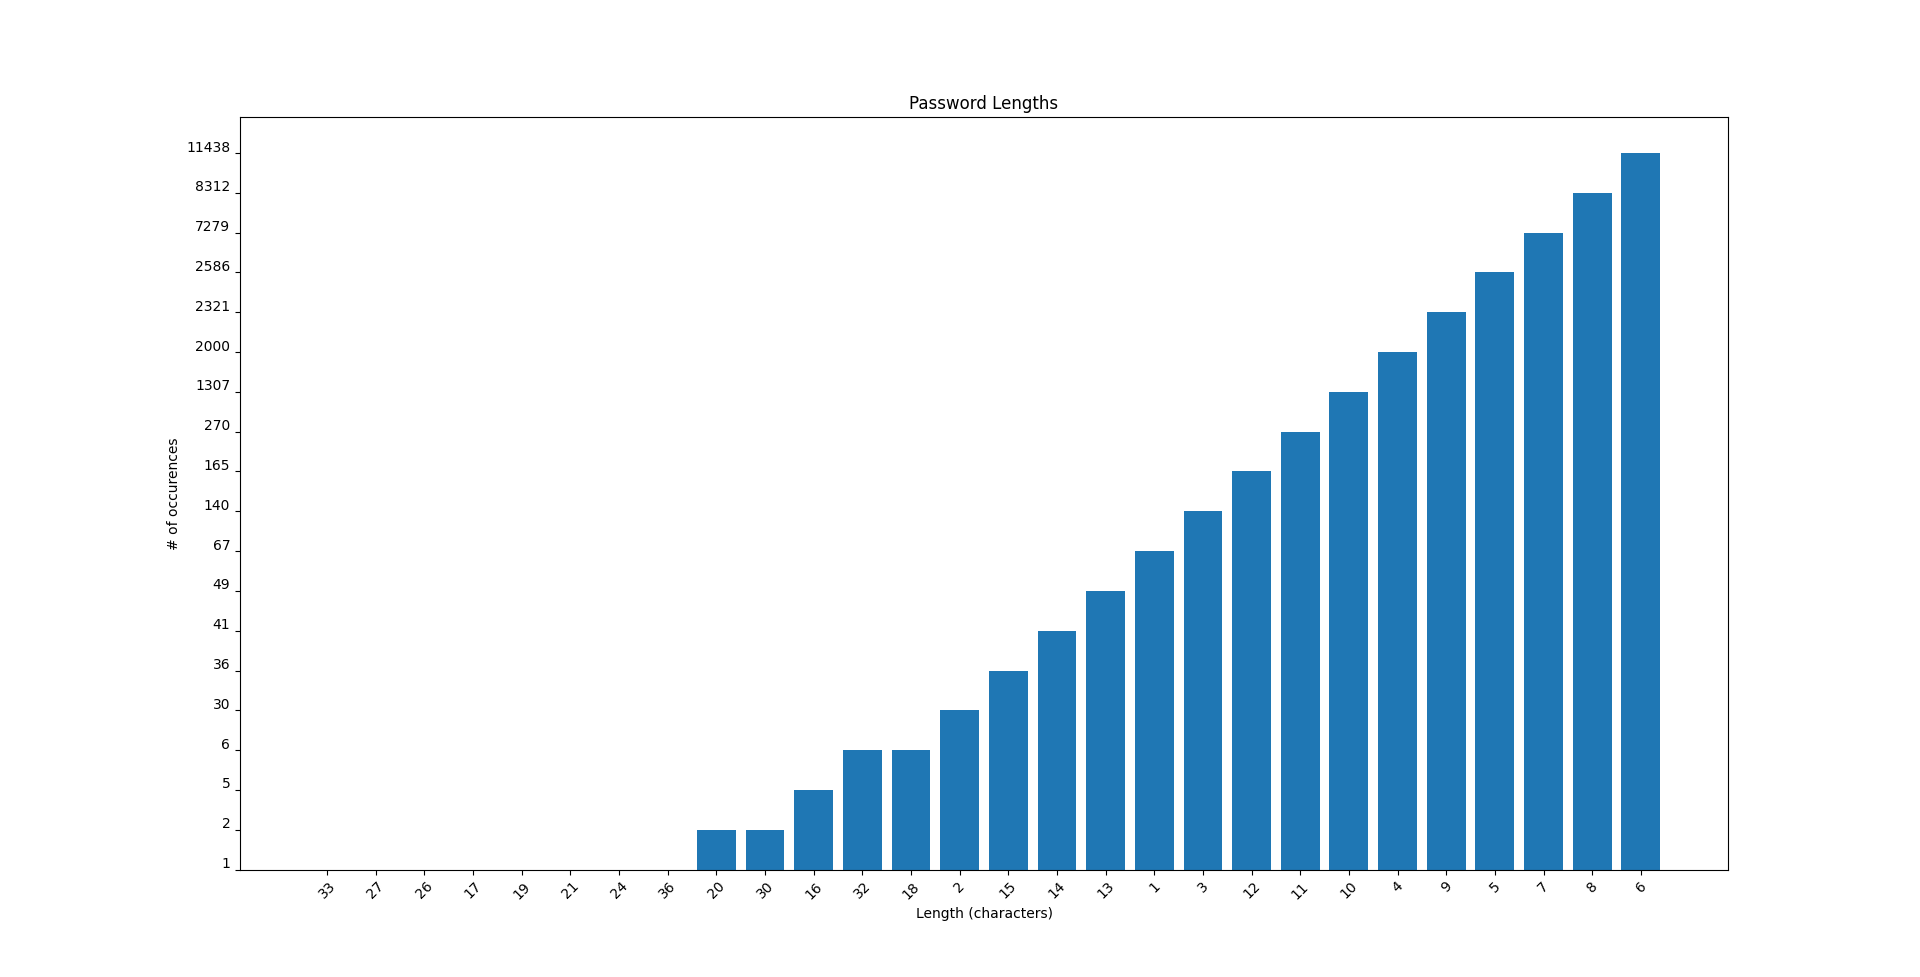
\includegraphics[width=1.8\textwidth]{password_length}
  \caption{Password Length}
  \label{fig:plen}
\end{figure}

\newpage
\subsection{What personal information is relevant for password guessing?}

To find the personal information, most relevant for password guessing, one of the password file was analysed manually. The file contained about 10,000 passwords, of which a little over 1,300 were categorised manually, with the help of a simple python script, which can be found in the Appendices (\ref{app:pwordcatscript}). To analyse these passwords, the script parsed over them, after which the researcher decided what category would suit the password best. The researcher then selected or entered the category, after which the script would increment the count on a category or create the category if it did not exist yet. This resulted in a number of categories. Most categories are self-explanatory, which is why not all will be explained in detail. The less evident categories will be handled along with the results.

\begin{figure}[!ht]
  \centering
  \hspace*{-4.3cm}
  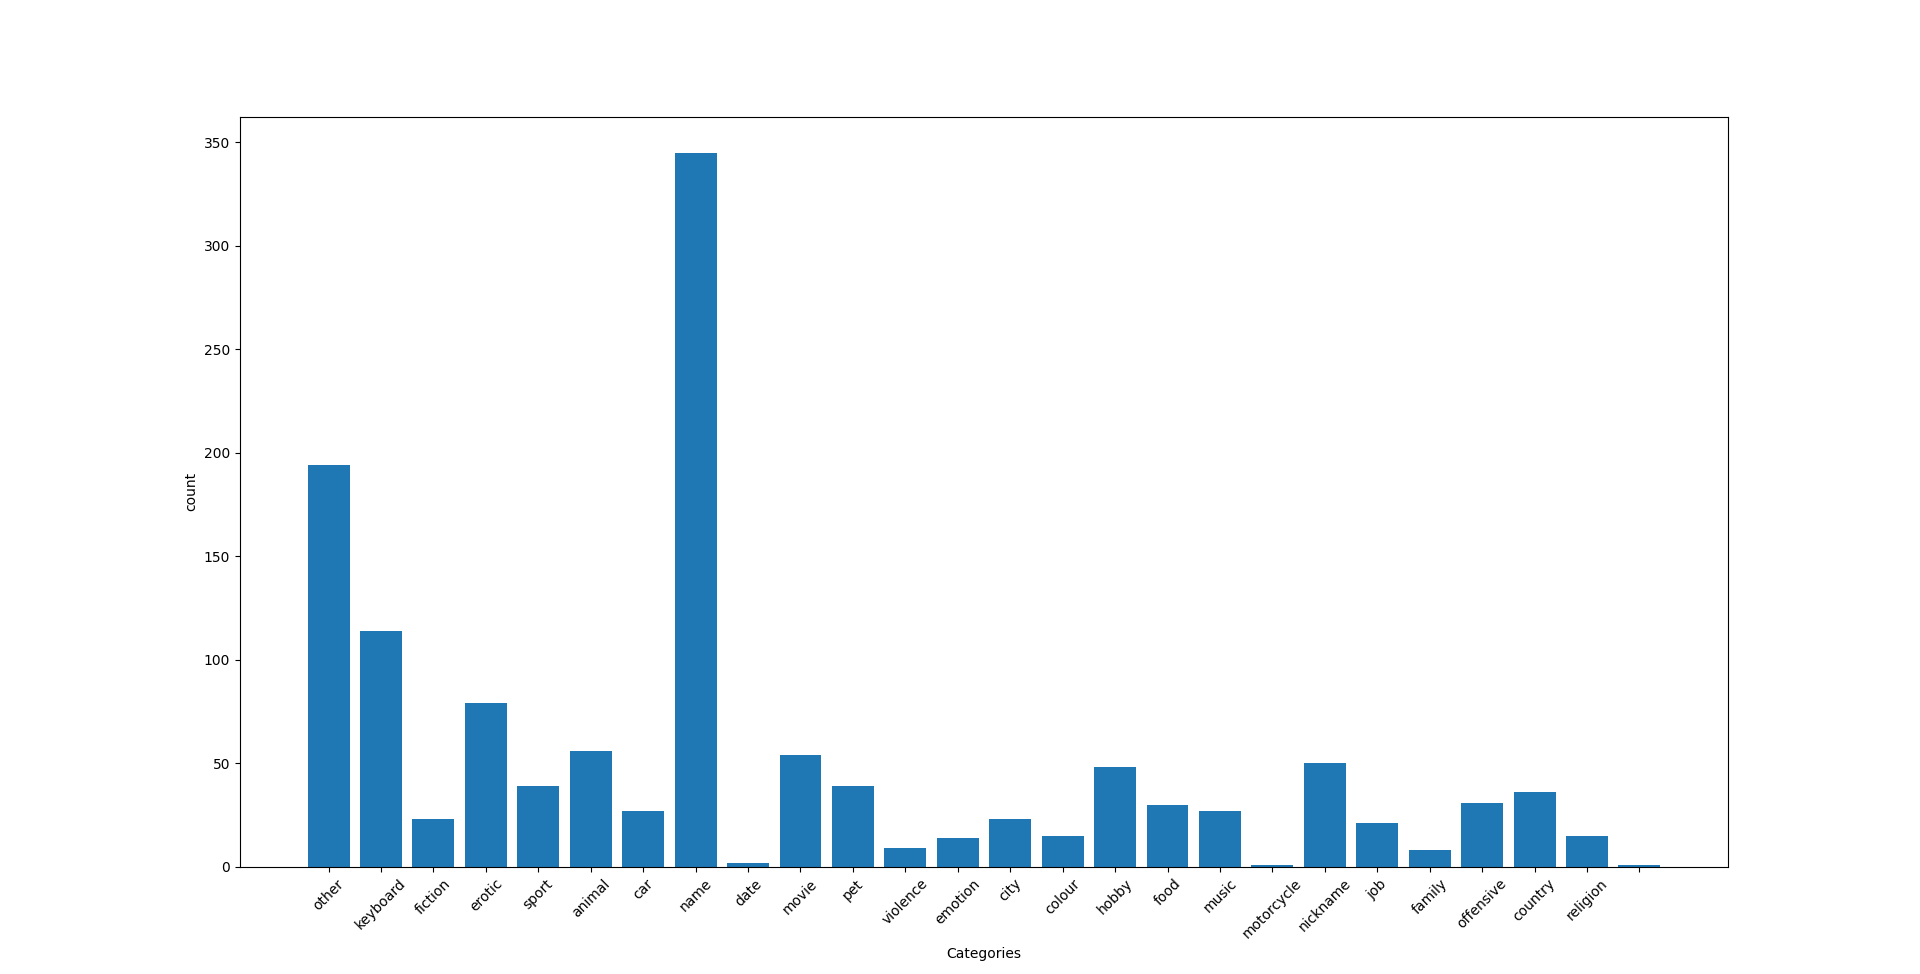
\includegraphics[width=1.7\textwidth]{password_categories}
  \caption{Password Categories}
  \label{fig:pcat}
\end{figure}

The results can be found in figure \ref{fig:pcat}. A number of categories are not entirely self-explanatory, which is why they will be explained in greater detail. The \lstinline{other} category includes all passwords that simply did not fit into any of the others, due to being passwords such as \lstinline{password} or \lstinline{mauyigv68}. Next to this, the \lstinline{keyboard} category can be seen, which holds all passwords that are clearly based on neighbouring keys or otherwise easy keystrokes. Some examples of this are \lstinline{qwerty} and \lstinline{mnbvcxz}.

The results show large differences between the count of the categories with the \lstinline{name} category being the one with the highest count by far, indicating that this category is important when trying to guess passwords. Since the \lstinline{other} category is a collection of all passwords that did not fit into any category, it is not surprising that this category has a high count. More surprising is the \lstinline{keyboard} category taking the third position, indicating that the patterns that are used for keystroke passwords should be investigated further.\\
The \lstinline{erotic} category also had a large number of passwords, which mostly seemed to have been created jokingly.\\

Other personal information that is often used is sport, like football clubs, baseball clubs, or simply the name of the sport.

\subsection{How can the processed information be structured efficiently, to allow for efficient dictionary attacks?}

Since using only the most popular format, with the most popular characters and password length would result in a password such as \lstinline{aaaaaa}, a different approach should be taken. To find the best method for generated passwords to be structured, a number of different approaches are described and compared based on positive and negative aspects.

\begin{itemize}
\item \textit{Generate maximum number of passwords, score passwords and sort according to score.}\\
  This method means to generate as many unique passwords as possible with a list of words, which are related to the target. Based on these words, henceforth called seed words, the program should try and create all possible combinations of the words, common practices, and common replacements of characters. Once this large number of passwords has been created, the passwords should be scored based on the found information. This means that the passwords should be scored for the format they use and how popular this format is, for the characters they use and how popular these characters are, and for the inclusion of words that belong to the found categories. Based on these scores, the passwords should be sorted. The highest scoring passwords should be on the top of the file, with decreasing scores following. This allows dictionary attacks to start with the most probable passwords to be correct. This method is likely to find the right password, as long as the right seed words are provided, although the computational costs are quite significant.\\
    
\item \textit{Generate fewer passwords, aiming specifically at a limited number of formats, score passwords and sort according to score.}\\
  This method would generate fewer passwords, but would follow the most popular formats. These passwords would then be scored and sorted much like the previous method. This method would allow for more aimed password generating, although a password would only need a slight deviation from these formats to avoid being guessed. For example, the top 8 formats are all shorter than 12 characters, meaning that a password would avoid being guessed accurately if the password is of a length of 12 or greater and the program only uses the top 8 formats.
\end{itemize}

The first method would be quite computationally heavy and on most systems, would probably take a while to finish. Also, this computation would become exponentially heavy with more seed words, due to more combinations being possible. The second method could be allowed to run much shorter, and could run on far less powerful equipment.\\
On the other hand, the first method will be very likely to generate the accurate password somewhere along the line, as long as the right seed words are provided. The second method will only provide the right password if one of the formats matches the password to be guessed. However, if this smaller list of passwords holds the right password, the increase in speed can be very significant, both when running the word-list generator and when running a dictionary attack.

\subsection{How can the program remain up to date with changing password practices?}
For the program to be able to remain up to date with changing password practices, it was researched if the research from the previous sub-questions could somehow be automated. The scripts, written for the research, were adjusted for this purpose and more password files were added to test if the output would be usable for the word-list generator. This resulted in a directory structure with raw password files in one directory and a script that wrote the results into a separate directory for the word-list generator to use, updating the formats, characters and passwords lengths.

\subsection{Sub-Conclusions of Password Pattern Research}

\begin{itemize}
\item What are standard password formats?\\

  The results provided valuable information on password formats, password lengths and the most used characters. The results show that passwords, with only lower-case alphabetical characters, a length of six characters, and using the most popular characters such as $a,e,r,o,i,n$, etc. are by far the most used ones. In a more general sense, the most used passwords consist of one type of character, which is either digits or alphabetical characters. Only a fraction of the used password formats mix lower-case alphabetical characters and digits, and a much smaller fraction uses different types of characters, although more than two different types in a single password format was not discovered in the data sets.
  
\item What personal information is relevant for password guessing?\\

  Looking at the results of categorising passwords, it becomes evident that most passwords are based on names, if based on any personal information. A large number of passwords are also based on keyboard strokes and erotic words/phrases. After this, most passwords are based on sport, animals, cars, movies, pets, nicknames and place of residence.
  
\item How can the processed information be structured efficiently, to allow for efficient dictionary attacks?\\

  When looking at the results, it can be seen that the different methods have different advantages and can be more useful than the other in different situations. One of the methods would require more computational power, but is most likely to find the right password, while the other method does not require such high computational power, but is less likely to include the right password.

\item How can the program remain up to date with changing password practices?\\

  By using scripts to analyse the password files and generate output that can be processed by the word-list generator, the program can be kept up to date. The user would need to place password files into the right directory and run the script, to update the most used formats, characters and password lengths.
  
\end{itemize}

\newpage
\section{Conclusions from Pattern Research}

The results provided useful insights into password formats, information used to keep passwords memorable, how information can be structured and processed and how the program can be kept up to date with changing password practices. Resulting from this, it becomes clear that the word-list generator should be able to find out what password formats are most popular, what characters are most used, and use this to score generated passwords. Since both mentioned methods for structuring and processing the data have their advantages and disadvantages, both should be used and be allowed to be enabled or disabled by configuration files. To stay up to date with changing password practices, the program should be capable of processing passwords automatically to generate the formats and most used characters, as done for this research. Users should also be able to provide the program with a list of words that relates to the target, preferably using information from the categories mentioned in this research.

\subsection{Recommendations for Future Research and Development}

To be able to score passwords more accurately, the researched categories should be used to discover what information is used in passwords. To be able to do this, it is recommended to include a number of lists in the program directories, where each category has a separate list. These lists can then be used to compare the contents to the passwords, scoring the generated passwords, based on the popularity of the category. For this reason, it is also recommended to automate the process of categorising password contents, although this would require massive amounts of data, a significant amount of development and Machine Learning-like programs to do accurately.

\newpage
\begin{thebibliography}{9}
\bibitem{bib:entro}
   Wanli Ma, John Campbell, Dat Tran, Dale Kleeman, Password Entropy and Password Quality, 2010, University of Canberra, Australia \texttt{https://ieeexplore.ieee.org/abstract/document/5635948}
 \bibitem{bib:pform}
   Hsien-Cheng Chou, Hung-Chang Lee, Hwan-Jeu Yu, Fei-Pei Lai, Kuo-Hsuan Huang, Chih-Wen Hsueh, Password Cracking Based On Learned Patterns From Disclosed Passwords, National Taiwan University, New Tapei City, Taiwan \texttt{http://www.ijicic.org/ijicic-11-12068.pdf}
 \bibitem{bib:seclists}
   Daniel Miessler, San Francisco, California, U.S.A \texttt{https://github.com/danielmiessler/SecLists/}
\end{thebibliography}

\newpage
\section{Appendices}

\subsection{Appendix A: SecLists}
\label{app:secl}

SecLists is a collection of data which is freely available on \href{https://github.com/danielmiessler/SecLists/}{Github}. It contains passwords, usernames and much more interesting data which can be used to gain insight in the most used passwords, their formats, used characters and password lengths.

\subsection{Appendix B: Python password format processor}
\label{app:pyprocc}

A Python 3 based script was written to simplify the processing of password data. The script was enabled to parse all data entered as files into a specific directory, splitting the task of processing each file into a separate child process (multiprocessing in Python). 

\begin{lstlisting}[language=Python]
#!/usr/bin/env python3

"""
To run this script successfully, place all files with leaked passwords in the 'passwords' directory. The output will be written to the 'form' directory.
"""

from multiprocessing import Process, Manager
import sys
import os
import time
from colorama import Fore, Back, Style
from datetime import datetime
import math

PATH = os.path.dirname(os.path.abspath(__file__))+'/'

def print_r_date(text):
    d = Back.BLUE+datetime.now().strftime('[%H:%M:%S]')+Style.RESET_ALL
    print('\033[K'+d+' '+text, end='\r')

def print_wdate(*args, **kwargs):
    d = Back.BLUE+datetime.now().strftime('[%H:%M:%S]')+Style.RESET_ALL
    print(d+' '.join(args), **kwargs)

def get_passwords(fd):
    """
    Get passwords from a file
    """
    passwds = []
    with open(fd, 'r') as fd:
        for passwd in fd:
            passwds.append(passwd.split(' ')[0])

    return passwds

def div_passwords(passwds, div_size):
    """
    """
    p_lists = []
    nr_divs = math.floor(len(passwds)/div_size)
    for i in range(nr_divs):
        p_lists.append(passwds[i*div_size:(i+1)*div_size])

    if len(passwds)>(nr_divs*div_size):
        p_lists.append(passwds[(nr_divs*div_size):])
    return p_lists

def exists_in_dict(dictio, key):
    """
    Check if a key exists in the dictionary.
    """
    for k, v in dictio.items():
        if k == key:
            return True
    return False

def sort_by_count(dictio):
    return {key: value for key, value in sorted(dictio.items(), key=lambda item: item[1])}

def passwd_file_to_format(forms_dict, lengths_dict, chars_dict, nchars_dict,
                          dchars_dict, schars_dict, passwds, fd, index,
                          pr_psswds):
    """
    Process to read file and create formats along with their counts
    """
    try:
        for passwd in passwds: # parse the lines in the file
            form = ''
            passwd = passwd.split('\n')[0]
            length = len(passwd)
            if length>0:
                for char in passwd:
                    if exists_in_dict(chars_dict, char):
                        chars_dict[char] +=1
                    else:
                        chars_dict[char] = 1
                    if char.isdigit():
                        form += 'd'
                        if exists_in_dict(dchars_dict, char):
                            dchars_dict[char] += 1
                        else:
                            dchars_dict[char] = 1
                    elif char.isalpha():
                        if exists_in_dict(nchars_dict, char):
                            nchars_dict[char] += 1
                        else:
                            nchars_dict[char] = 1
                        if char.isupper():
                            form += 'C'
                        else:
                            form += 'c'
                    else:
                        form += 's'
                        if exists_in_dict(schars_dict, char):
                            schars_dict[char] += 1
                        else:
                            schars_dict[char] = 1
                        

                if exists_in_dict(forms_dict, form): # check if the format already exists in the dict
                    forms_dict[form] += 1
                else:
                    forms_dict[form] = 1
                if exists_in_dict(lengths_dict, length): # check if the length already exists in the dict
                    lengths_dict[length] += 1
                else:
                    lengths_dict[length] = 1
            if exists_in_dict(pr_psswds, 'done'):
                pr_psswds['done'] += 1
            else:
                pr_psswds['done'] = 1
        print_wdate(Fore.GREEN+'--['+str(index)+']--'+Style.RESET_ALL+'Finished process for', fd.name)
    except Exception as e:
        print(Fore.RED+'[ERROR]'+Style.RESET_ALL+' process unsuccessful')
        print(Fore.RED+str(e)+Style.RESET_ALL)

dir_psswd = PATH+'passwords' # directory where standard password wordlists are stored
dir_output = PATH+'processed' # directory where the processed output will be stored
file_form = 'format.txt' # file name of the file where password formats will be stored
file_len = 'length.txt' # file name of the file where password lengths will be stored
file_char = 'char.txt' # file name of the file where used chars will be stored
file_schar = 'schar.txt' # file name of the file where used special chars will be stored
file_dchar = 'dchar.txt' # file name of the file where used digit chars will be stored
file_nchar = 'nchar.txt' # file name of the file where used normal chars will be stored
max_prccs = 500
div_size = 4000
feedback_time = 5

files = os.scandir(dir_psswd) # All files in the 'passwords' directory as a generator for efficiency

processes = [] # List of processes to deal with reading the files
forms_dict = Manager().dict() # Dictionary to hold the formats and their count
lengths_dict = Manager().dict() # Dictionary to hold password lengths and their count
chars_dict = Manager().dict() # Dictionary to hold used characters and their count
schars_dict = Manager().dict() # Dictionary to hold used special characters and their count
dchars_dict = Manager().dict() # Dictionary to hold used digit characters and their count
nchars_dict = Manager().dict() # Dictionary to hold used normal characters and their count
pr_psswds = Manager().dict()

nr_passwds=0
nr_prccs=0
for f in files: # parse the files
    print(Fore.YELLOW+'...Parsing:'+f.name+Style.RESET_ALL)
    psswds = get_passwords(f)
    nr_passwds += len(psswds)
    p_lists = div_passwords(psswds, div_size)
    print(Fore.YELLOW+'### '+Style.RESET_ALL+'Starting', len(p_lists), 'processes for',
          Fore.YELLOW+f.name+Style.RESET_ALL)
    for p_list in p_lists:
        nr_prccs += 1
        print_wdate(Fore.GREEN+'--['+str(nr_prccs)+']--'+Style.RESET_ALL, end='')
        print(f.name, len(p_list), 'passwords')
        processes.append(Process(target=passwd_file_to_format, args=(forms_dict,
                                                                     lengths_dict,
                                                                     chars_dict,
                                                                     nchars_dict,
                                                                     dchars_dict,
                                                                     schars_dict,
                                                                     p_list,f,nr_prccs,
                                                                     pr_psswds)))
print('Processing', nr_passwds)
pr_psswds['total'] = nr_passwds
        
# Check if not too many processes will be running
if nr_prccs >= max_prccs:
    print(Fore.RED, '[ERROR]', Style.RESET_ALL,
          'Too many files/passwords to process with separate processes. '\
          'Please lower amount of processes. This might slow the program down,'\
          ' but will allow it to run. Maximum processes:', max_prccs,
          'Current number is', nr_prccs)
    sys.exit(1)

start_time = time.time() # start time of the processes
for process in processes:
    process.start()

# Update user on processes that are still running
running = True
running_time = time.time()
try:
    while running:
        running=False
        ctr=0
        indexes=[]
        for process in processes:
            ctr+=1
            if process.is_alive():
                indexes.append(str(ctr))
                running=True
        if time.time()-running_time>feedback_time:
            print_r_date(Fore.GREEN+str(pr_psswds['done'])+'/'+str(pr_psswds['total'])+Fore.YELLOW+ \
                         '('+str(int(pr_psswds['done']/pr_psswds['total']*100))+'%)'+ \
                         '--Still running:'+ \
                         Fore.CYAN + \
                         ','.join(indexes[:10])+'...'+Style.RESET_ALL)
            running_time = time.time()
            time.sleep(1)
            print_r_date(Fore.GREEN+str(pr_psswds['done'])+'/'+str(pr_psswds['total'])+Fore.YELLOW+ \
                         '('+str(int(pr_psswds['done']/pr_psswds['total']*100))+'%)'+ \
                         '--Still running:'+ \
                         Fore.CYAN + \
                         ','.join(indexes[:10])+'...'+Style.RESET_ALL)
except KeyboardInterrupt:
    print('Exiting')
    sys.exit(0)
        
# Ensure safe exit for all processes
for process in processes:
    process.join()

print(Fore.GREEN, '\n[SUCCESS]', Style.RESET_ALL, 'Sorting the results\n')

# Sort results in their respective files
forms_dict=sort_by_count(forms_dict)
lengths_dict=sort_by_count(lengths_dict)
chars_dict=sort_by_count(chars_dict)
nchars_dict=sort_by_count(nchars_dict)
dchars_dict=sort_by_count(dchars_dict)
schars_dict=sort_by_count(schars_dict)

with open(dir_output+'/'+file_form, 'w') as fd:
    print(Fore.YELLOW+'### '+Style.RESET_ALL+'Writing to', fd.name)
    for form, count in forms_dict.items():
        fd.write(form+' '+str(count)+'\n')

with open(dir_output+'/'+file_len, 'w') as fd:
    print(Fore.YELLOW+'### '+Style.RESET_ALL+'Writing to', fd.name)
    for length, count in lengths_dict.items():
        fd.write(str(length)+' '+str(count)+'\n')

with open(dir_output+'/'+file_char, 'w') as fd:
    print(Fore.YELLOW+'### '+Style.RESET_ALL+'Writing to', fd.name)
    for char, count in chars_dict.items():
        fd.write(str(char)+' '+str(count)+'\n')

with open(dir_output+'/'+file_nchar, 'w') as fd:
    print(Fore.YELLOW+'### '+Style.RESET_ALL+'Writing to', fd.name)
    for nchar, count in nchars_dict.items():
        fd.write(str(nchar)+' '+str(count)+'\n')

with open(dir_output+'/'+file_dchar, 'w') as fd:
    print(Fore.YELLOW+'### '+Style.RESET_ALL+'Writing to', fd.name)
    for dchar, count in dchars_dict.items():
        fd.write(str(dchar)+' '+str(count)+'\n')

with open(dir_output+'/'+file_schar, 'w') as fd:
    print(Fore.YELLOW+'### '+Style.RESET_ALL+'Writing to', fd.name)
    for schar, count in schars_dict.items():
        fd.write(str(schar)+' '+str(count)+'\n')

# Display time it took to complete processes in seconds
print(Fore.YELLOW+'Processed',nr_passwds,'in', int(time.time()-start_time),
      'seconds'+Style.RESET_ALL)
\end{lstlisting}

\subsection{Appendix C: Python graph plotter}
\label{app:pyplot}

To create a new overview for the processed data, a Python script was written to create plots of the data. The script is listed below.

\begin{lstlisting}[language=Python]
#!/usr/bin/env python3

import sys
import os
from colorama import Fore, Style
import matplotlib.pyplot as plt

try:
    choice = sys.argv[1]
except:
    print(Fore.RED+'[ERROR]'+Style.RESET_ALL,
          'Wrong number of parameters')
    sys.exit(1)

dir_output = 'processed'
files = os.scandir(dir_output)
fd_choice = ''

for fd in files:
    if choice in fd.name:
        print(fd.name)
        fd_choice = dir_output+'/'+fd.name
        break

if fd_choice == '':
    print(Fore.RED+'[ERROR]'+Style.RESET_ALL,
          'Something went wrong with the filename')
    sys.exit(1)
    
x=[]
y=[]
    
with open(fd_choice, 'r') as fd:
    for line in fd:
        line=line.split(' ')
        x.append(line[0])
        y.append(line[1])

while len(x) > 100:
    x=x[int(len(x)/4):]
    y=y[int(len(y)/4):]

plt.bar(x,y)
plt.xlabel(choice)
plt.ylabel('count')
if len(x[0]) > 1:
    plt.xticks(rotation=45)
    if len(x[0]) > 2:
        plt.xticks(rotation=90)
           
plt.show()
\end{lstlisting}

\subsection{Appendix D: Used Password File Names}
\label{app:pwordfile}

\begin{itemize}
\item 10k-most-common.txt
\item probable-v2-top12000.txt
\item unkown-azul.txt
\item clarkson-university-82.txt
\item stupid-ones-in-production.txt
\item darkweb2017-top10000.txt
\item twitter-banned.txt
\end{itemize}

\subsection{Appendix E: Password Categorising Script}
\label{app:pwordcatscript}
To (slightly) ease the categorising of personal information used in passwords, the script below was used, which parsed passwords in the file, until reaching the end or until C-c was used to exit. Allows user to create a new category for a password or use an existing one. Each time a category is selected, the count increments. At the end, a graph is produced.

\begin{lstlisting}
#!/usr/bin/env python3
import sys
import os
from colorama import Fore, Style
import matplotlib.pyplot as plt

pfile = 'passwords/10k-most-common.txt'
passwords = []

with open(pfile, 'r') as fd:
    lines = fd.readlines()
    for line in lines:
        passwords.append(line.split('\n')[0])

categories = {
}

try:
    for password in passwords:
        print(password)
        index=0
        existing = ''
        for key, value in categories.items():
            existing += ', '+key+'<'+str(index)+'>'
            index += 1
        print('Existing categories:', existing)
        choice = input('Choose category for '+Fore.GREEN+password+Style.RESET_ALL+': ')
        if choice.isdigit():
            print(choice)
            if len(list(categories)) > int(choice):
                key = list(categories)[int(choice)]
                print(key)
            else:
                print('Does not exist yet. Skipping...')
        else:
            key = choice
        if key in categories:
            categories[key] += 1
        else:
            categories[key] = 1
except KeyboardInterrupt:
    print('Making graph')

x = [key for key, value in categories.items()]
y = [value for key, value in categories.items()]

plt.bar(x,y)
plt.xlabel('Categories')
plt.ylabel('count')
plt.xticks(rotation=45)
           
plt.show()
\end{lstlisting}

\end{document}
